\chapter{Vũ trụ học Newton và phương trình Friedmann}

Lần trước chúng ta đã nói về metric của không gian. Câu hỏi tiếp theo là động lực học: thừa số tỉ lệ thay đổi theo thời gian như thế nào? Trước hết là một chút hình học, rồi đến vũ trụ học Newton. Phương trình Friedmann lúc này vẫn chưa được suy ra từ thuyết tương đối rộng. Nó sẽ được suy ra từ các phương trình của Newton.

\section{Tính đồng nhất, tính đẳng hướng và metric phụ thuộc thời gian}

Tính đồng nhất và tính đẳng hướng là các giả thiết luôn được đặt ra. Nếu vũ trụ đồng nhất, đẳng hướng và biến đổi theo thời gian, thì định luật Hubble luôn đúng. Ở bất kỳ thời điểm cố định nào, vận tốc lùi xa tỉ lệ với khoảng cách,
\begin{equation}
v = H(t)\,d.
\end{equation}
Sự tỉ lệ ấy là tuyến tính. Cái không đổi ở đây không phải là theo thời gian, mà là theo không gian: tại một thời điểm cho trước, cùng một hệ số tỉ lệ áp dụng ở khắp mọi nơi.

\begin{classroomqa}
\audiencequestion{Có nghĩa là tỉ lệ tuyến tính phải không?}\lecturetimestamp{00:02:06}
\lecturerresponse{Đúng. Ở một thời điểm cố định, vận tốc lùi xa tỉ lệ tuyến tính với khoảng cách. Hệ số tỉ lệ đó là hằng số Hubble. Nói chung nó phụ thuộc vào thời gian, nhưng không biến thiên từ điểm này sang điểm khác trong không gian.}
\end{classroomqa}

Đó là lý do vì sao cụm từ ``hằng số Hubble'' dễ gây hiểu lầm. Nó là hằng theo vị trí trong không gian. Nó không phải là hằng theo thời gian.

Tiếp theo là một câu hỏi tự nhiên. Nếu không gian giãn nở, tại sao các thước mét lại không giãn nở theo? Câu trả lời là các thước mét được giữ với nhau bởi những lực mạnh hơn khổng lồ so với bất cứ thứ gì gắn với sự giãn nở vũ trụ ở thang nguyên tử. Các vật liên kết thì vẫn liên kết. Cái giãn nở là khoảng cách giữa những vật đủ tách rời nhau, chẳng hạn các thiên hà cách nhau đủ xa đến mức chúng không liên kết nhau đủ mạnh.

\begin{classroomqa}
\audiencequestion{Có vấn đề gì liên quan đến việc các thước đo cũng đang giãn nở không?}\lecturetimestamp{00:04:00}
\lecturerresponse{Không. Các thước đo không giãn nở. Các tọa độ mới giãn nở. Những lực giữ các thước mét gắn kết với nhau mạnh hơn rất nhiều so với các hiệu ứng do sự giãn nở gây ra, nên các vật liên kết thông thường không giãn nở cùng nền. Các thiên hà đủ xa nhau thì tách ra, nhưng thước mét thì không.}
\end{classroomqa}

Thậm chí người ta còn có thể hình dung một hiệu ứng đẩy bổ sung rất nhỏ giữa các nguyên tử. Nhưng ngay cả thế nó cũng không xé rời một cái thước. Nó chỉ làm dịch khoảng cách cân bằng đi một chút, giống như một lực kéo thêm rất nhỏ làm thay đổi vị trí cân bằng của một lò xo cứng.

\begin{classroomqa}
\audiencequestion{Nhưng không thể mô hình hóa nó như một lực giữa các điểm, có đúng không? Vì nếu không thì nó sẽ là một gia tốc.}\lecturetimestamp{00:05:29}
\lecturerresponse{Có thể hình dung một lực bổ sung nhỏ giữa các nguyên tử, nhưng nếu nó rất nhỏ so với các lực liên kết thì nó chỉ làm dịch vị trí cân bằng đi chút ít. Bản thân sự giãn nở không tạo ra một định luật lực thông thường. Một số kiểu giãn nở có thể được mô hình hóa bằng lực, cụ thể là sự giãn nở có gia tốc, nhưng đó là một câu hỏi để sau.}
\end{classroomqa}

Vì vậy, các tọa độ hữu ích là những tọa độ được gắn vào phân bố vật chất đang giãn nở. Những thiên hà không có thêm chuyển động riêng thì giữ nguyên các giá trị tọa độ. Cái thay đổi theo thời gian là quan hệ giữa độ tách tọa độ và khoảng cách vật lý đo bằng mét. Quan hệ đó được mã hóa bởi thừa số tỉ lệ \(a(t)\).

Đối với không gian phẳng, metric không gian có thể viết là
\begin{equation}
ds^2 = a(t)^2\left(dx^2+dy^2+dz^2\right).
\end{equation}
Ở đây \(a\) là khoảng cách thực, đo bằng mét, giữa các điểm lân cận cách nhau một đơn vị khoảng cách tọa độ. Nếu vũ trụ giãn nở, \(a\) trở thành đại lượng phụ thuộc thời gian.

Để chuyển sang không-thời gian, hãy bắt đầu từ dạng của thuyết tương đối hẹp
\begin{equation}
d\tau^2 = dt^2 - ds^2,
\end{equation}
rồi thế metric không gian vào. Ta được
\begin{equation}
d\tau^2 = dt^2 - a(t)^2\left(dx^2+dy^2+dz^2\right).
\end{equation}
Các hệ số không phụ thuộc vào vị trí trong không gian. Chúng chỉ phụ thuộc vào thời gian. Đó là phát biểu của tính đồng nhất bằng ngôn ngữ metric. Metric đường chéo có dạng
\begin{equation}
g_{\mu\nu}=\mathrm{diag}\!\left(1,-a(t)^2,-a(t)^2,-a(t)^2\right).
\end{equation}
\editorialnote{Ma trận đường chéo đầy đủ được viết ở đây bám theo phần mô tả tensor metric bằng lời nói quanh 00:14:33. Khung hình trên bảng cho thấy rõ phần tử độ dài, nhưng ma trận không hiện ra đủ rõ để đọc hoàn toàn.}

Không có các hạng ngoài đường chéo. Không có \(dx\,dy\), không có \(dx\,dt\), cũng không có hạng hỗn hợp nào khác. Metric gần như đơn giản như metric của không-thời gian phẳng. Điểm đặc biệt là chính quan hệ giữa độ đo không gian và thời gian lại phụ thuộc thời gian.

\begin{figure}
\centering
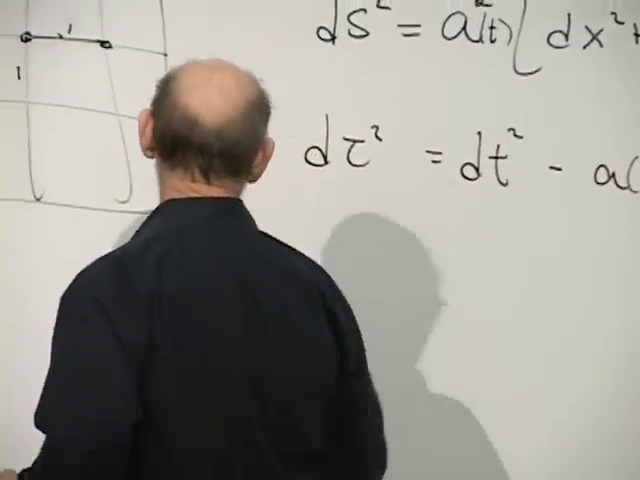
\includegraphics[width=0.62\textwidth]{lecture_02_figure_02.png}
\caption{Phác họa lưới đồng chuyển động và khoảng không-thời gian với một thừa số tỉ lệ phụ thuộc thời gian.}
\end{figure}

Hình vẽ truyền đạt đúng ý chính. Alice và Bob vẫn cách nhau một đơn vị trong các tọa độ đồng chuyển động, nhưng một đơn vị tọa độ ấy biểu thị ngày càng nhiều mét hơn khi thời gian trôi đi. Nếu \(a(t)\) bằng 0 vào một thời điểm nào đó trong quá khứ, thì mọi độ tách vật lý đều sẽ bằng 0. Mọi thứ sẽ bị ép chồng lên nhau. Đó là lý do vì sao \(a\to 0\) tương ứng với mật độ vô hạn. Nếu \(a\) tăng, vũ trụ trở nên ngày càng loãng hơn.

Dạng này của metric không đúng trong mọi hệ quy chiếu. Đây là dạng trong hệ quy chiếu chuyển động cùng các thiên hà.

\begin{classroomqa}
\audiencequestion{Trong phương trình đó, cái \(t\) nhỏ, \(a(t)\), thì \(t\) đó là thời gian của ai?}\lecturetimestamp{00:19:19}
\lecturerresponse{Đó là thời gian được đo bởi các đồng hồ chuyển động cùng các thiên hà. Hãy hình dung những chiếc đồng hồ giống hệt nhau được chế tạo trong cùng một xưởng đồng hồ vũ trụ và được các thiên hà mang theo. Trong hệ quy chiếu này, biến thời gian chính xác là đại lượng mà các đồng hồ ấy đo. Dọc theo đường thế giới của một thiên hà, thời gian riêng trùng với thời gian tọa độ này.}
\end{classroomqa}

Thật vậy, dọc theo đường thế giới của một thiên hà đồng chuyển động,
\begin{equation}
dx=dy=dz=0,
\end{equation}
nên
\begin{equation}
d\tau^2 = dt^2,
\end{equation}
và do đó
\begin{equation}
dt=d\tau.
\end{equation}

\begin{classroomqa}
\audiencequestion{Có những phép biến đổi nào giữ cho dạng này của metric bất biến không?}\lecturetimestamp{00:23:08}
\lecturerresponse{Các phép quay thì có, vì \(dx^2+dy^2+dz^2\) bất biến dưới các phép quay. Nhưng các phép boost Lorentz không bảo toàn dạng này. Chính vật chất đã chọn ra hệ quy chiếu chuyển động cùng các thiên hà, và trong một hệ quy chiếu khác thì thế giới sẽ không còn trông đẳng hướng nữa.}
\end{classroomqa}

\section{Một vật phóng trong trường hấp dẫn}

Trước khi áp dụng Newton cho toàn bộ vũ trụ, sẽ hữu ích nếu lùi lại một bài toán đơn giản hơn: một khối lượng lớn \(M\), một khối lượng nhỏ hơn nhiều \(m\), và một xung ban đầu hướng ra ngoài. Sau xung đó, vật nhỏ đơn giản chuyển động trong trường hấp dẫn và làm đúng điều Newton bảo nó phải làm.

Đối với cuộc thảo luận vũ trụ học, điều quan trọng không phải là toàn bộ bài toán quỹ đạo. Điều quan trọng là sự bảo toàn năng lượng. Động năng là
\begin{equation}
\frac{1}{2}mv^2.
\end{equation}

\begin{figure}
\centering
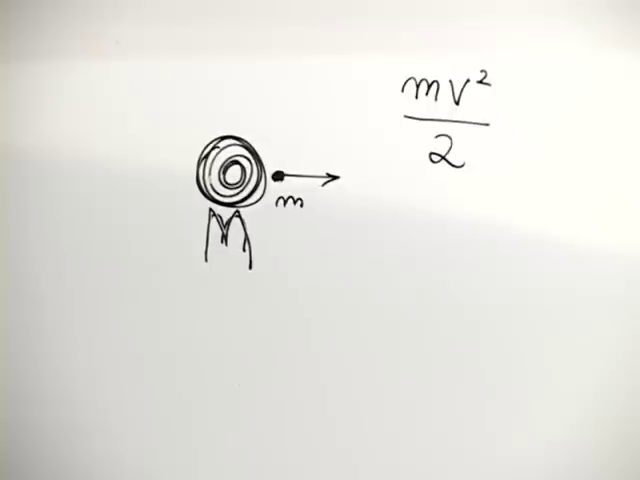
\includegraphics[width=0.42\textwidth]{lecture_02_figure_03.png}
\caption{Vật thử đi ra ngoài và hạng động năng \(\frac{1}{2}mv^2\).}
\end{figure}

Thế năng hấp dẫn chứa tích của các khối lượng, hằng số Newton, và một lũy thừa bậc nhất của khoảng cách ở mẫu số. Trong cách viết trên bảng, các thừa số xuất hiện theo thứ tự \(mMG/D\), nên tốt nhất ở đây cũng giữ nguyên thứ tự đó:
\begin{equation}
-\frac{mMG}{D}.
\end{equation}
Vì vậy tổng năng lượng là
\begin{equation}
\frac{1}{2}mv^2-\frac{mMG}{D}.
\end{equation}
Bảo toàn năng lượng chỉ nói rằng đại lượng này không đổi theo thời gian đối với hạt cụ thể đang được xét. Các hạt khác nhau có thể có những năng lượng khác nhau.

\begin{figure}
\centering
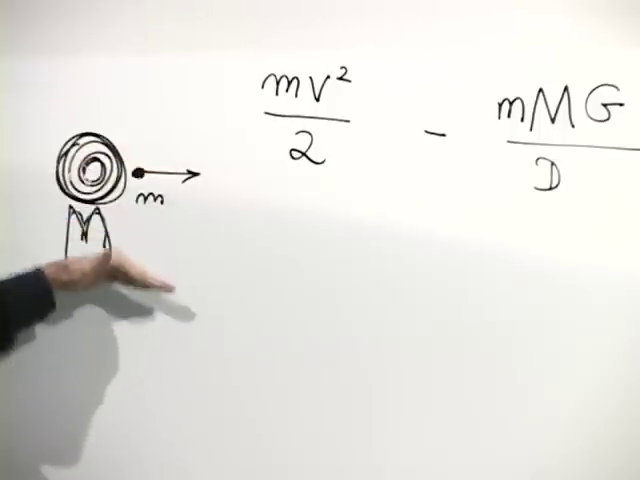
\includegraphics[width=0.62\textwidth]{lecture_02_figure_04.png}
\caption{Tổng năng lượng Newton của một vật thử chuyển động theo phương bán kính: hạng động năng trừ thế năng hấp dẫn.}
\end{figure}

Dấu âm là quan trọng. Thế năng hấp dẫn là âm vì lực hấp dẫn là lực hút. Đưa hạt lại gần hơn tạo ra một lượng thế năng âm lớn hơn về độ lớn. Đưa nó ra xa hơn làm cho thế năng bớt âm đi.

\begin{classroomqa}
\audiencequestion{Thế năng tăng theo khoảng cách chứ không giảm sao?}\lecturetimestamp{00:34:13}
\lecturerresponse{Đúng. Hãy quên các hằng số đi và nhìn vào các đồ thị của \(1/D\) và \(-1/D\). Lực tác dụng theo chiều làm thế năng giảm. Vì vậy, một lực hút tương ứng với đường cong lật ngược, \(-1/D\), nên thế năng tăng theo khoảng cách và trở nên âm hơn khi hạt đi vào trong.}
\end{classroomqa}

\begin{figure}
\centering
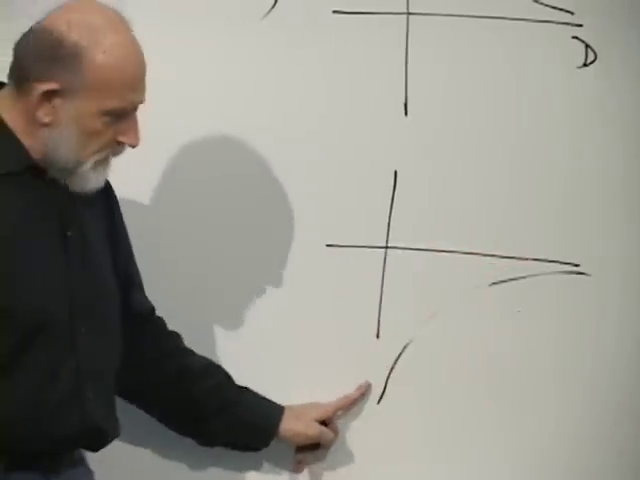
\includegraphics[width=0.46\textwidth]{lecture_02_figure_05.png}
\caption{So sánh định tính giữa \(1/D\) và \(-1/D\) đối với dấu của thế năng hấp dẫn.}
\end{figure}

\section{Vận tốc thoát}

Bây giờ hãy phân loại các khả năng. Năng lượng có thể dương, âm hoặc bằng 0. Chỉ có ba trường hợp đó.

\begin{itemize}
\item Nếu năng lượng âm, hạt bị liên kết. Ném nó lên với vận tốc quá nhỏ thì nó đi lên, chậm dần, quay đầu, rồi rơi trở lại.
\item Nếu năng lượng dương, hạt thoát ra. Lúc đầu trọng lực làm nó chậm lại, nhưng không đủ để dừng nó, và cuối cùng nó đi ra xa với một vận tốc tiệm cận hướng ra ngoài khác không.
\item Nếu năng lượng đúng bằng không, hạt ở đúng vận tốc thoát. Đó là trường hợp biên giữa thoát ra và không thoát ra.
\end{itemize}

Với vận tốc ban đầu đủ nhỏ, hạng thế năng chi phối ngay từ đầu và năng lượng là âm.

\begin{figure}
\centering
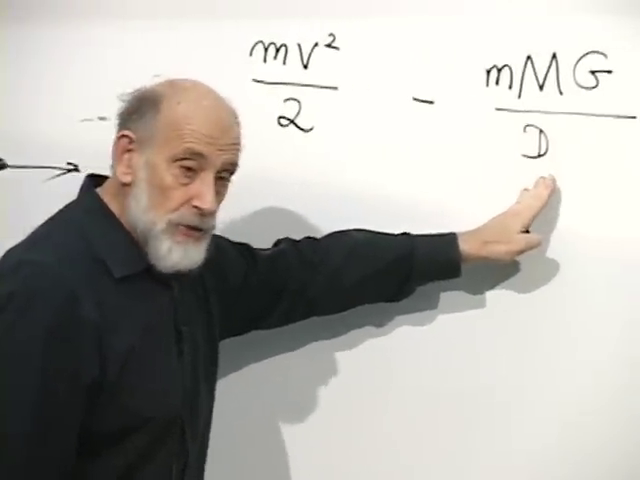
\includegraphics[width=0.62\textwidth]{lecture_02_figure_06.png}
\caption{Khi vận tốc hướng ra ngoài nhỏ, hạng thế năng âm chi phối tổng năng lượng.}
\end{figure}

Trong trường hợp năng lượng bằng không, khoảng cách tiếp tục tăng, nhưng độ lớn vận tốc tiếp tục giảm. Hạt không thể đứng yên ở bất kỳ thời điểm hữu hạn nào. Nếu có, nó sẽ rơi trở lại. Vì vậy khoảng cách là không bị chặn, còn vận tốc thì tiến dần về 0.

Đây là phép tương tự trực tiếp có ý nghĩa đối với vũ trụ học. Vũ trụ có thể ứng xử theo cùng cách đó. Nếu dòng Hubble hướng ra ngoài ban đầu đủ lớn, mọi thứ đều thoát khỏi mọi thứ khác. Nếu nó quá nhỏ, trọng lực thắng thế và sẽ có một vụ co sụp khổng lồ. Cũng có trường hợp biên, hoàn toàn tương tự với vận tốc thoát.

\section{Định lý Newton}

Phép quy giản trong vũ trụ học hoạt động được là nhờ định lý Newton đối với định luật nghịch đảo bình phương.

Nếu vật chất được phân bố đối xứng cầu quanh một tâm nào đó, thì lực hấp dẫn tác dụng lên một hạt ở bên ngoài phân bố ấy hoàn toàn giống hệt như thể toàn bộ khối lượng đều tập trung tại tâm. Nhưng định lý còn mạnh hơn thế. Nếu hạt ở bên trong phân bố, thì chỉ phần khối lượng ở bán kính nhỏ hơn mới góp phần. Khối lượng ở bán kính lớn hơn không tạo ra hợp lực nào.

Phiên bản sáng sủa nhất của định lý là trường hợp vỏ mỏng. Một vỏ cầu hoàn hảo không tác dụng lực hấp dẫn nào lên một hạt ở bất kỳ đâu bên trong nó, kể cả khi hạt không ở tâm. Thoạt nhìn điều đó có vẻ đáng ngạc nhiên, nhưng nó đúng đối với định luật \(1/r^2\).

\begin{classroomqa}
\audiencequestion{Trong ví dụ thầy nêu ở đó, liệu ta có nên hơi ngạc nhiên khi dường như lúc hạt đi qua biên thì lực lại gián đoạn không?}\lecturetimestamp{00:48:19}
\lecturerresponse{Có. Với một vỏ lý tưởng mỏng vô hạn, điều đó quả là đáng ngạc nhiên, và đó là điều đặc biệt của định luật lực \(1/r^2\). Một vỏ thực có bề dày, nên sự biến thiên được làm trơn đi, nhưng mệnh đề sắc nét đối với vỏ lý tưởng chính là tính chất đáng chú ý của định lý Newton.}
\end{classroomqa}

Khi ấy, một hình vẽ sẽ làm cho định lý có vẻ hợp lý. Hãy thay một khối lượng điểm bằng một nguồn nước điểm. Trong ba chiều, dòng chảy hướng ra ngoài giảm như \(1/r^2\). Hãy đặt liên tục các nguồn như vậy khắp trên một vỏ cầu. Ở bên ngoài vỏ, dòng chảy trông đúng hệt như thể mọi thứ đều tập trung tại tâm. Ở bên trong vỏ, không thể có dòng tổng cộng nào, vì không có nguồn ở tâm. Chính cấu trúc ấy là nền tảng của định lý hấp dẫn.

Mục đích ở đây không phải là chứng minh lại định lý, mà là vận dụng nó.

\section{Vũ trụ đồng nhất như một bài toán một vật}

Bây giờ quay lại vũ trụ học. Hãy lấy một vùng nhỏ của vũ trụ, được lấp đầy bởi một chất khí thiên hà đồng đều. Nếu muốn, ta có thể đặt mình ở tâm. Điều đó chỉ là một sự tiện lợi. Bất kỳ ai cũng có thể tự xem mình ở tâm, và vẫn phải thu được cùng một phương trình.

Hãy chọn một thiên hà trên trục \(x\) tại tọa độ đồng chuyển động \(x\). Vì vũ trụ đẳng hướng, việc chọn trục nào không quan trọng. Vẽ một mặt cầu có tâm tại \(x=0\) và đi qua thiên hà đó. Theo định lý Newton, lực tác dụng lên thiên hà hoàn toàn giống hệt như thể toàn bộ khối lượng bên trong mặt cầu ấy đều tập trung ở tâm, còn mọi thứ bên ngoài thì không đóng góp gì.

Mặt cầu ấy giãn nở cùng với các thiên hà. Nó luôn chứa cùng những thiên hà đó, và vì thế cùng một tổng khối lượng, mặc dù bán kính vật lý của nó thay đổi theo thời gian.

Vì thế, chuyển động của thiên hà đó tuân theo đúng cùng một kiểu phương trình năng lượng như vật phóng:
\begin{equation}
\frac{1}{2}mv^2-\frac{mMG}{D}=\text{constant}.
\end{equation}
Ở đây, \(M\) bây giờ có nghĩa là khối lượng bên trong mặt cầu đang giãn nở, chứ không phải khối lượng tâm trong hình minh họa ban đầu. Đại số khi đó được đơn giản hóa bằng cách nhân với \(2\) rồi chia cho \(m\). Vì một hằng số chia cho \(m\) vẫn chỉ là một hằng số, ta có thể viết
\begin{equation}
v^2-\frac{2MG}{D}=\text{constant}.
\end{equation}
Một lần nữa, ``hằng số'' có nghĩa là hằng theo thời gian đối với thiên hà cụ thể đó.

Bây giờ hãy liên hệ điều này với thừa số tỉ lệ. Khoảng cách vật lý tới thiên hà là
\begin{equation}
D=ax,
\end{equation}
vì \(x\) là một tọa độ đồng chuyển động cố định. Vận tốc của nó là
\begin{equation}
v=\dot D=\dot a\,x.
\end{equation}

Khối lượng bên trong mặt cầu bằng mật độ nhân với thể tích. Nếu \(\rho\) là mật độ khối lượng, thì
\begin{equation}
M=\frac{4\pi}{3}\rho D^3=\frac{4\pi}{3}\rho a^3x^3.
\end{equation}
Thay vào phương trình năng lượng, ta được
\begin{equation}
\dot a^2x^2-\frac{2G}{ax}\left(\frac{4\pi}{3}\rho a^3x^3\right)=\text{constant},
\end{equation}
hay
\begin{equation}
\dot a^2x^2-\frac{8\pi G}{3}\rho a^2x^2=\text{constant}.
\end{equation}

Cả hai hạng ở vế trái đều tỉ lệ với \(x^2\). Mọi thứ khác ở đó đều như nhau ở khắp mọi nơi. Vì thế vế phải cũng phải tỉ lệ với \(x^2\). Điều đó không mâu thuẫn với việc gọi nó là một hằng số. Nó có nghĩa là hằng theo thời gian đối với mỗi \(x\) cố định, nhưng từ thiên hà này sang thiên hà khác nó vẫn có thể tỉ lệ theo \(x^2\). Điều đó hợp lý. Những thiên hà ở xa hơn chuyển động nhanh hơn.

Vậy hãy khử nhân tử chung \(x^2\). Hằng số còn lại bây giờ không phụ thuộc cả thời gian lẫn không gian. Hãy viết nó theo cách chuẩn về mặt lịch sử là \(-k\):
\begin{equation}
\dot a^2-\frac{8\pi G}{3}\rho a^2=-k.
\end{equation}
Sau khi chia cho \(a^2\),
\begin{equation}
\left(\frac{\dot a}{a}\right)^2=\frac{8\pi G}{3}\rho-\frac{k}{a^2}.
\end{equation}

Đây là phương trình Friedmann-Robertson-Walker nổi tiếng, mặc dù bài giảng cũng nhận xét rằng thực ra nó là phương trình của Friedman. Quy ước dấu là do lịch sử. Việc viết \(-k\) không có nghĩa là \(k\) phải dương. \(k\) có thể dương, âm hoặc bằng không. Trong các đơn vị mà tốc độ ánh sáng được đặt bằng \(1\), \(k\) là vô thứ nguyên.

\section{Mật độ và phương trình do vật chất chi phối}

Câu hỏi tiếp theo đến ngay lập tức: \(\rho\) là gì? Nó không phải là một hằng số. Khi vũ trụ giãn nở, mật độ giảm.

Để biểu diễn sự phụ thuộc đó, hãy xét một khối lập phương đơn vị trong không gian tọa độ: mỗi cạnh dài một đơn vị theo \(x\), \(y\) và \(z\). Cùng những thiên hà ấy vẫn nằm trong khối lập phương đó ở mọi thời điểm vì nó giãn nở cùng với các tọa độ. Vì vậy khối lượng bên trong khối lập phương tọa độ ấy là cố định.

\editorialnote{Bài giảng dùng lại ký hiệu \(M\) ở vài chỗ. Ở đây \(M_{\Box}\) chỉ được dùng để phân biệt khối lượng trong một khối lập phương đơn vị của không gian tọa độ với khối lượng tâm trước đó và khối lượng chứa trong mặt cầu.}

Độ dài cạnh vật lý của khối lập phương là \(a\), nên thể tích vật lý của nó là \(a^3\). Do đó
\begin{equation}
\rho=\frac{M_{\Box}}{a^3}.
\end{equation}
Đây là trường hợp vật chất chi phối: vế phải chỉ chứa mật độ của vật chất thông thường, phi tương đối tính.

\begin{classroomqa}
\audiencequestion{Theo phương trình đó, hằng số Hubble là một hàm của \(\rho\). Vì thế nó không phải là một hằng số.}\lecturetimestamp{01:19:21}
\lecturerresponse{Chính xác. Hằng số Hubble thực ra không hằng. Nó phụ thuộc vào mật độ, mà mật độ lại thay đổi theo thời gian. Bài giảng thậm chí còn đùa rằng bài thi cuối kỳ có thể chỉ gồm một câu hỏi: Hằng số Hubble có phải là một hằng số không?}
\end{classroomqa}

Thay \(\rho=M_{\Box}/a^3\) vào phương trình Friedmann cho
\begin{equation}
\left(\frac{\dot a}{a}\right)^2=\frac{8\pi G M_{\Box}}{3a^3}-\frac{k}{a^2}.
\end{equation}

Đến đây các lựa chọn tùy ý đã rõ. Cần có khối lượng trong một khối lập phương đơn vị của không gian tọa độ và giá trị của \(k\). Ba dấu có thể có của \(k\) tương ứng với ba trường hợp năng lượng của bài toán vật phóng.

\begin{itemize}
\item Nếu \(-k>0\), thì về mặt hiệu dụng năng lượng tương ứng với trường hợp vượt vận tốc thoát, và vũ trụ giãn nở mãi mãi.
\item Nếu \(-k<0\), trọng lực cuối cùng sẽ thắng thế và vũ trụ co sụp trở lại.
\item Nếu \(k=0\), vũ trụ đúng bằng vận tốc thoát.
\end{itemize}

\begin{classroomqa}
\audiencequestion{Nếu \(k=0\) thì vận tốc giữa hai thiên hà đang tiến dần về 0, đúng không?}\lecturetimestamp{01:21:12}
\lecturerresponse{Đúng. Trong trường hợp tới hạn, vận tốc tiến dần về 0, nhưng khoảng cách vẫn là không bị chặn. Các thiên hà vẫn tiếp tục tách xa nhau, chỉ là ngày càng chậm hơn. Nếu chúng thực sự đứng yên tại một thời điểm hữu hạn nào đó, chúng sẽ rơi trở lại.}
\end{classroomqa}

\section{Trường hợp tới hạn \(k=0\)}

Bây giờ hãy chọn trường hợp đơn giản nhất, \(k=0\). Đó chính là trường hợp vận tốc thoát chính xác, và nó đơn giản hơn chỉ vì toán học đơn giản hơn. Phương trình trở thành
\begin{equation}
\left(\frac{\dot a}{a}\right)^2=\frac{8\pi G M_{\Box}}{3a^3}.
\end{equation}

Vế phải luôn dương và không bao giờ bằng không. Vì thế \(\dot a/a\) không thể đi qua 0. Trong trường hợp này, vũ trụ không thể quay đầu. Nó hoặc luôn giãn nở, hoặc luôn co lại. Hãy lấy nhánh giãn nở.

Bây giờ hãy đoán một định luật lũy thừa,
\begin{equation}
a(t)=ct^p.
\end{equation}
Khi đó
\begin{equation}
\dot a = cp\,t^{p-1},
\end{equation}
nên
\begin{equation}
\frac{\dot a}{a}=\frac{p}{t}.
\end{equation}
Thay vào phương trình vi phân, ta được
\begin{equation}
\frac{p^2}{t^2}=\frac{8\pi G M_{\Box}}{3c^3t^{3p}}.
\end{equation}
Để các lũy thừa của \(t\) khớp nhau, phải có
\begin{equation}
3p=2.
\end{equation}
Vậy
\begin{equation}
p=\frac{2}{3}.
\end{equation}
Khi đó các hằng số phải thỏa mãn
\begin{equation}
\frac{4}{9}=\frac{8\pi G M_{\Box}}{3c^3},
\end{equation}
suy ra
\begin{equation}
c^3=6\pi G M_{\Box}.
\end{equation}
Do đó
\begin{equation}
a(t)=\left(6\pi G M_{\Box}\right)^{1/3}t^{2/3}.
\end{equation}

Vẫn còn có thể có một độ dời cộng tính của thời gian. Có thể hấp thụ nó bằng cách thay \(t\) bởi \(t-t_0\). Một khi chọn gốc thời gian sao cho \(a=0\) tại \(t=0\), hằng số còn lại đó biến mất.

Vậy vũ trụ giãn nở theo lũy thừa hai phần ba của thời gian,
\begin{equation}
a(t)\propto t^{2/3}.
\end{equation}
Nó không giãn nở tuyến tính theo thời gian. Sự tăng tuyến tính sẽ là tương tự của chuyển động không gia tốc. Ở đây sự giãn nở chậm dần.

Nếu ngoại suy công thức lùi về \(t=0\), thừa số tỉ lệ đi về 0 và mật độ phân kỳ. Phát biểu \(a=0\) là một cực hạn. Chúng ta không biết điều gì xảy ra với vật chất khi nó trở nên quá đậm đặc. Điểm thực sự là ở một giai đoạn sớm nào đó, mọi thứ đều chen chúc đến mức các nguyên tử, hạt nhân và quark đều bị nhồi chặt vào nhau trong một trạng thái có mật độ cực kỳ lớn.

\section{Hằng số Hubble và tuổi của vũ trụ}

Trong mô hình tới hạn,
\begin{equation}
H(t)=\frac{\dot a}{a}=\frac{2}{3t}.
\end{equation}
Vì vậy, hằng số Hubble xấp xỉ bằng nghịch đảo của tuổi vũ trụ,
\begin{equation}
t=\frac{2}{3H}.
\end{equation}
Đây là một trong những thành quả chính của phép tính này. Đo hằng số Hubble ngày nay, ta sẽ thu được một ước lượng về tuổi của vũ trụ, ít nhất là lùi về đến điểm mà mô hình Newton không còn có ý nghĩa nữa.

Tuổi được nêu vào khoảng \(13\) đến \(14\) tỷ năm. Văn bản cũng nói rằng việc lấy \(k=0\) là rất phù hợp về mặt quan sát: ở mức độ chính xác được nêu ở đó, chưa biết có độ lệch đáng kể nào khỏi \(k=0\).

\begin{classroomqa}
\audiencequestion{Tôi chỉ hơi chưa rõ \(M\) và \(a\) là gì.}\lecturetimestamp{01:39:16}
\lecturerresponse{Cả hai đều chứa tính tùy ý do cách chọn lưới tọa độ. Thay hộp quy ước thì lượng vật chất trong đó thay đổi, và giá trị số của thừa số tỉ lệ cũng thay đổi theo. Đại lượng vật lý là mật độ, \(M/a^3\), hay tương đương là các tổ hợp như \(a/M^{1/3}\) không phụ thuộc vào cách chọn lưới. Trong nghiệm \(k=0\), hằng số chưa biết nhân với \(t^{2/3}\) bị triệt tiêu khỏi \(\dot a/a\), nên hệ thức tuổi \(t=2/3H\) không phụ thuộc vào khối lượng của hộp quy ước.}
\end{classroomqa}

Sự triệt tiêu đó thấy ngay trong nghiệm. Nếu
\begin{equation}
a(t)=Ct^{2/3},
\end{equation}
thì
\begin{equation}
\dot a=\frac{2}{3}Ct^{-1/3},
\end{equation}
và do đó
\begin{equation}
\frac{\dot a}{a}=\frac{2}{3t}.
\end{equation}
Hằng số \(C\) bị khử hoàn toàn.

\section{Vì sao phép suy dẫn theo Newton lại đúng}

Về cuối, câu hỏi trở thành: vì sao phép suy dẫn theo Newton lại phù hợp với phép suy dẫn tương đối tính đến thế?

\begin{classroomqa}
\audiencequestion{Tất cả điều này dường như phụ thuộc vào giả thiết về một vũ trụ mở.}\lecturetimestamp{01:45:44}
\lecturerresponse{Ở giai đoạn này, phép suy dẫn là theo Newton, mà vật lý Newton có nghĩa là không gian phẳng. Cách diễn giải \(k\) theo hình học của không gian được để sang bài giảng sau. Ở đó \(k=0\) sẽ tương ứng với không gian phẳng, còn các dấu khác sẽ gắn với hình học không gian cong.}
\end{classroomqa}

\begin{classroomqa}
\audiencequestion{Ở một thời điểm nào đó rất lâu trong quá khứ, độ dài của các thước mét có phụ thuộc vào \(a\) không?}\lecturetimestamp{01:47:53}
\lecturerresponse{Lùi đủ xa về quá khứ, vật chất sẽ dày đặc đến mức các thước mét riêng rẽ thật ra sẽ không tồn tại. Trước khi đến mức ấy, chúng sẽ bị ép sát vào nhau. Bài giảng cũng nhắc chúng ta rằng dù sao thuyết tương đối cũng không cho phép các vật thật sự cứng tuyệt đối: nếu một vật cứng hoàn toàn, một cú đẩy ở một phía sẽ truyền tín hiệu sang phía kia tức thời, nhanh hơn ánh sáng.}
\end{classroomqa}

\begin{classroomqa}
\audiencequestion{Vì sao thầy nghĩ lại có sự trùng hợp này giữa các phương trình Newton và tương đối tính?}\lecturetimestamp{01:49:03}
\lecturerresponse{Bởi vì cách xử lý theo Newton chỉ được áp dụng cho một vùng đủ nhỏ. Miễn là vùng đó nhỏ so với bán kính độ cong của toàn bộ vũ trụ, và miễn là các vận tốc Hubble cục bộ ở đó nhỏ hơn nhiều so với tốc độ ánh sáng, thì cơ học Newton là một xấp xỉ tốt. Bài giảng so sánh điều này với việc nghiên cứu cỏ mọc trên Trái Đất: ta có thể hiểu quá trình cục bộ mà không cần dùng đến độ cong của toàn bộ Trái Đất.}
\end{classroomqa}

Đây là logic của vùng cục bộ. Cơ học Newton giả định, thứ nhất, rằng độ cong của không gian không quan trọng đối với vấn đề đang xét, và thứ hai, rằng không có gì trong vùng cục bộ chuyển động gần tốc độ ánh sáng. Trong vũ trụ học, điều đó có nghĩa là chọn một vùng đủ lớn để đồng nhất, nhưng vẫn đủ nhỏ để các hiệu ứng độ cong là không đáng kể và các vận tốc Hubble vẫn phi tương đối tính.

Với điều đó trong đầu, phép tính Newton không phải là ngẫu nhiên. Nó là xấp xỉ cục bộ của một phương trình mà cũng có thể được đọc dưới dạng tương đối tính. Nếu chuyển hạng độ cong sang vế trái, phương trình Friedmann trở thành
\begin{equation}
\left(\frac{\dot a}{a}\right)^2+\frac{k}{a^2}=\frac{8\pi G}{3}\rho.
\end{equation}
Vế trái mang tính hình học: nó chứa thừa số tỉ lệ và, trong buổi sau, độ cong của không gian. Vế phải là mật độ năng lượng. Đó chính xác là loại phương trình người ta chờ đợi từ thuyết tương đối rộng.

Lần tới, chủ đề sẽ là bản thân độ cong, các phương trình Einstein, và mối liên hệ giữa phép suy dẫn tương đối tính đó với phép suy dẫn theo Newton.